\documentclass[11pt,english]{article}

%%%%%%%%%%%%%%%%%%%%%%%%%%%%%%%%%%%%%%%%%%%%%%%%%%%%%%%%%%%
% Packages
%%%%%%%%%%%%%%%%%%%%%%%%%%%%%%%%%%%%%%%%%%%%%%%%%%%%%%%%%%%

% paper size & margins
\usepackage{fullpage}
\usepackage[showframe=false,margin=1in]{geometry}
\parindent=0pt

% font management
\usepackage{relsize}
\usepackage[T1]{fontenc} % for properly hyphenating words with accented chars
\usepackage[latin1]{inputenc}
\usepackage{babel}

% math
\usepackage{amsmath}
\usepackage{amsthm}
\usepackage{amssymb}
\usepackage{textcomp}
\usepackage{stmaryrd}
\usepackage{upgreek}
\usepackage{bm}
\usepackage[linesnumbered,ruled,vlined]{algorithm2e}

% assorted
\usepackage{url}
\usepackage{breakurl}
\usepackage{xspace}
\usepackage{comment}
\usepackage{color}
\usepackage{xcolor}
\usepackage{afterpage}
\usepackage{graphicx}
\usepackage{hyperref}
\usepackage{pdfpages}
\usepackage{subcaption}
\usepackage{multirow}
\usepackage{placeins}
\usepackage{listings}
\usepackage{dsfont}
\usepackage{mathtools}

%%%%%%%%%%%%%%%%%%%%%%%%%%%%%%%%%%%%%%%%%%%%%%%%%%%%%%%%%%%
% Shortcuts
%%%%%%%%%%%%%%%%%%%%%%%%%%%%%%%%%%%%%%%%%%%%%%%%%%%%%%%%%%%
\newcommand{\hide}[1]{}

\usepackage{environ}
\usepackage{xparse}

\ExplSyntaxOn
\NewEnviron{bmatrixT}
{
\marine_transpose:V \BODY
}

\int_new:N \l_marine_transpose_row_int
\int_new:N \l_marine_transpose_col_int
\seq_new:N \l_marine_transpose_rows_seq
\seq_new:N \l_marine_transpose_arow_seq
\prop_new:N \l_marine_transpose_matrix_prop
\tl_new:N \l_marine_transpose_last_tl
\tl_new:N \l_marine_transpose_body_tl

\cs_new_protected:Nn \marine_transpose:n
{
\seq_set_split:Nnn \l_marine_transpose_rows_seq { \\ } { #1 }
\int_zero:N \l_marine_transpose_row_int
\prop_clear:N \l_marine_transpose_matrix_prop
\seq_map_inline:Nn \l_marine_transpose_rows_seq
{
\int_incr:N \l_marine_transpose_row_int
\int_zero:N \l_marine_transpose_col_int
\seq_set_split:Nnn \l_marine_transpose_arow_seq { & } { ##1 }
\seq_map_inline:Nn \l_marine_transpose_arow_seq
{
\int_incr:N \l_marine_transpose_col_int
\prop_put:Nxn \l_marine_transpose_matrix_prop
{
\int_to_arabic:n { \l_marine_transpose_row_int }
,
\int_to_arabic:n { \l_marine_transpose_col_int }
}
{ ####1 }
}
}
\tl_clear:N \l_marine_transpose_body_tl
\int_step_inline:nnnn { 1 } { 1 } { \l_marine_transpose_col_int }
{
\int_step_inline:nnnn { 1 } { 1 } { \l_marine_transpose_row_int }
{
\tl_put_right:Nx \l_marine_transpose_body_tl
{
\prop_item:Nn \l_marine_transpose_matrix_prop { ####1,##1 }
\int_compare:nF { ####1 = \l_marine_transpose_row_int } { & }
}
}
\tl_put_right:Nn \l_marine_transpose_body_tl { \\ }
}
\begin{bmatrix}
    \l_marine_transpose_body_tl
\end{bmatrix}
}
\cs_generate_variant:Nn \marine_transpose:n { V }
\cs_generate_variant:Nn \prop_put:Nnn { Nx }
\ExplSyntaxOff


\definecolor{codewhite}{rgb}{0.95,0.95,0.95}
\definecolor{codegreen}{rgb}{0,0.6,0}
\definecolor{codegray}{rgb}{0.5,0.5,0.5}
\definecolor{codepurple}{rgb}{0.58,0,0.82}
\definecolor{backcolour}{rgb}{0.1,0.1,0.1}

\lstdefinestyle{mystyle}{
    backgroundcolor=\color{backcolour},
    commentstyle=\color{codegreen},
    keywordstyle=\color{orange},
    numberstyle=\tiny\color{codegray},
    stringstyle=\color{codepurple},
    basicstyle=\ttfamily\scriptsize\color{codewhite},
    breakatwhitespace=false,
    breaklines=true,
    captionpos=b,
    keepspaces=true,
    numbers=left,
    numbersep=5pt,
    showspaces=false,
    showstringspaces=false,
    showtabs=false,
    tabsize=2
}

\lstset{style=mystyle}

\DeclarePairedDelimiter\abs{\lvert}{\rvert}%
\DeclarePairedDelimiter\norm{\lVert}{\rVert}%

\makeatletter
\let\oldabs\abs
\def\abs{\@ifstar{\oldabs}{\oldabs*}}
%
\let\oldnorm\norm
\def\norm{\@ifstar{\oldnorm}{\oldnorm*}}
\makeatother


%%%%%%%%%%%%%%%%%%%%%%%%%%%%%%%%%%%%%%%%%%%%%%%%%%%%%%%%%%%
% Title / Author
%%%%%%%%%%%%%%%%%%%%%%%%%%%%%%%%%%%%%%%%%%%%%%%%%%%%%%%%%%%
\begin{document}

    \title{CS7643: Deep Learning \\
    Fall 2019\\ HW4 Solutions}
    \author{Nicolas \textsc{Six}}
    \maketitle


    %%%%%%%%%%%%%%%%%%%%%%%%%%%%%%%%%%%%%%%%%%%%%%%%%%%%%%%%%%%
    % Body
    %%%%%%%%%%%%%%%%%%%%%%%%%%%%%%%%%%%%%%%%%%%%%%%%%%%%%%%%%%%

    \section{Optimal Policy and Value Function}
    \subsection{Always stay policy}
    
If this function has a minimum, it has to be when its partial derivative regarding to $\vec{w}$ is null.
In addition, as the this function is convex, so admit only one point where $\vec{w}$ is null, and so only one extrema.
As this function is clearly unbounded from above this extrema is the global minimum.

\begin{align*}
    \frac{\partial \left( f\left( \vec{w^{(t)}} \right) +
                           \left< \vec{w} - \vec{w^{(t)}}, \nabla f\left( \vec{w^{(t)}} \right) \right>
                           + \frac{\lambda}{2} \left\| \vec{w} - \vec{w^{(t)}} \right\|^2 \right)
    }{
        \partial \vec{w}
    }
    &= 0 \\
    \Leftrightarrow
    \frac{\partial \left(
                           \left< \vec{w}, \nabla f\left( \vec{w^{(t)}} \right) \right> \right) }
    {\partial \vec{w}} +
    \frac{\partial \left( \frac{\lambda}{2} \left< \vec{w} - \vec{w^{(t)}}, \vec{w} - \vec{w^{(t)}} \right> \right) }
    {\partial \vec{w}}
    &= 0 \\
    \Leftrightarrow
    \left< \frac{\partial\vec{w}}{\partial\vec{w}}, \nabla f\left( \vec{w^{(t)}} \right) \right> +
    \lambda \left< \frac{\partial\vec{w}}{\partial\vec{w}}, \vec{w} - \vec{w^{(t)}} \right>
    &= 0 \\
    \Leftrightarrow
    \left< \frac{\partial\vec{w}}{\partial\vec{w}}, \nabla f\left( \vec{w^{(t)}} \right) + \lambda \left( \vec{w} - \vec{w^{(t)}} \right) \right>
    &= 0 \\
    \Leftrightarrow
    \nabla f\left( \vec{w^{(t)}} \right) + \lambda \left( \vec{w} - \vec{w^{(t)}} \right)
    &= \vec{0} \\
    \Leftrightarrow
    \vec{w}
    &= \vec{w^{(t)}} - \frac{1}{\lambda} \nabla f\left( \vec{w^{(t)}} \right) \\
\end{align*}

In conclusion we get the following:

\begin{align*}
    \vec{w^*} &= \vec{w^{(t)}} - \frac{1}{\lambda} \nabla f\left( \vec{w^{(t)}} \right) \\
    \eta &= \frac{1}{\lambda}
\end{align*}

This show us that under our current set of assumption, the gradient descent is leading us the the optimal solution.

    \pagebreak
    \subsection{Optimal policy}
    The optimal policy is $("go","go")$.
Lets name this policy $\pi^*$.
Now we can compute the value of each state following this policy.

\begin{align*}
    V^*(S_2) &= r(S_2, "go") \\
    &= 3
    V^*(S_1) &= r(S_1, "go") + \gamma V^*(S_2) \\
    &= -2 + 3 \gamma
\end{align*}




    \pagebreak
    \subsection{Value function}
    

\begin{align*}
    V^0 &= [0,0] \\
    V^1 &= [-1,3] \\
    V^2 &= [1,3] \\
    V^3 &= [1,3] \\
    V^* &= [1,3]
\end{align*}


    \pagebreak
    \section{Value Iteration Convergence}
    \subsection{Error decrease}
    
\begin{align*}
    \left\| V^0 - V^* \right\|_\infty &= 3 \\
    \left\| V^1 - V^* \right\|_\infty &= 2 \\
    \left\| V^2 - V^* \right\|_\infty &= 0 \\
    \left\| V^3 - V^* \right\|_\infty &= 0 \\
\end{align*}

We can see that the error of the value iteration is decreasing monotonically in this example.



    \pagebreak
    \subsection{Proof of decrease over iterations}
    
Our current model with three different weights value can only represent linear separation of the data.
With $W$ representing the slope of the slope of this line in the plan formed by the two variable $x$ and $y$ and the
bias $b$ representing the shift regarding to the origin.

\begin{figure}[h!]
    \begin{center}
        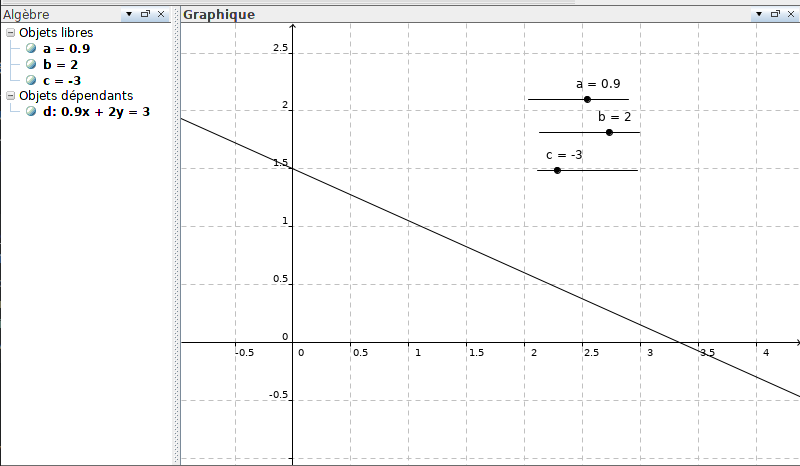
\includegraphics[width=.6\linewidth]{../2_logic_XOR/xor_graph.png}
        \caption{Representation of the the frontier depending on the three weights}
    \end{center}
\end{figure}

But to get an XOR we need to satisfy the following conditions:

\begin{align*}
    f(0,0) &< 0 \\
    f(0,1) &\geq 0 \\
    f(1,0) &\geq 0 \\
    f(1,1) &< 0
\end{align*}

Which is strictly impossible with only one linear boundary.

As a side not it's important to note that:

\[
    XOR(x, y) = \left( \overline{x} \cdot y \right) + ( x \cdot \overline{y} )
\]

So it's possible to have XOR with linear classifier as we already showed how to get $AND$ and $OR$ operations
in subsection \ref{2.1}.
The $NOT$ operation being just a simple one input classifier with one weight of negative value and a small positive bias.





    \pagebreak
    \subsection{Proof of bound}
    Starting with the previous results, we have:

\begin{align*}
    \left\| T(V^n) - T(V^{n+1}) \right\|_{\infty} &\leq \gamma \left\| V^{n} - V^{n+1} \right\|_{\infty} \\
    \Leftrightarrow
    \left\| V^{n+1} - V^{n+2} \right\|_{\infty} &\leq \gamma \left\| V^{n} - V^{n+1} \right\|_{\infty} \\
    \Leftrightarrow
    \left\| V^{n+1} - V^* \right\|_{\infty} - \left\| V^{n+2} - V^* \right\|_{\infty} &\leq \gamma \left\| V^{n} - V^{n+1} \right\|_{\infty} \\
    \Leftrightarrow
    \left\| V^{n+1} - V^* \right\|_{\infty} - \left\| T(V^{n+1}) - T(V^*) \right\|_{\infty} &\leq \gamma \left\| V^{n} - V^{n+1} \right\|_{\infty} \\
    \Leftrightarrow
    \left\| V^{n+1} - V^* \right\|_{\infty} - \gamma \left\| V^{n+1} - V^* \right\|_{\infty} &\leq \gamma \left\| V^{n} - V^{n+1} \right\|_{\infty} \\
    \Leftrightarrow
    (1 - \gamma) \left\| V^{n+1} - V^* \right\|_{\infty} &\leq \gamma \left\| V^{n} - V^{n+1} \right\|_{\infty} \\
    \Leftrightarrow
    \left\| V^{n+1} - V^* \right\|_{\infty} &\leq \frac{\gamma}{1 - \gamma} \left\| V^{n} - V^{n+1} \right\|_{\infty} \\
    \Leftrightarrow
    \left\| V^{n+1} - V^* \right\|_{\infty} &\leq \frac{\gamma}{1 - \gamma} \epsilon \text{ for } n > N
\end{align*}



    \pagebreak
    \subsection{Unique fixed point}
    


\begin{align}
    \left\| T(x_1) - T(x_2) \right\|_{\infty} &\leq \gamma \left\| x_1 - x_2 \right\|_{\infty} \label{2.4bonus_eq}
\end{align}


From equation \ref{2.4bonus_eq} we know that $T$ is continuous, monotonic and decreasing (as $0 \leq \alpha < 1$).

So the hyper plan designed by $T$ must intersect with the hyper plan designed by the identity function, which is continuous, monotonic and increasing.

In addition, if there is two different fixed point, $x^{*1}$ and $x^{*2}$, then:

\begin{align*}
    \left\| T(x^{*1}) - T(x^{*2}) \right\|_\infty
    &= \left\| x^{*1} - x^{*2} \right\|_\infty \\
    &\geqslant \alpha \left\| x^{*1} - x^{*2} \right\|_\infty \text{ as } \alpha < 1 \text{ and } \left\| x^{*1} - x^{*2} \right\|_\infty \neq 0
\end{align*}

So we can't have two distinct fixed points for $T$.

In conclusion, there is one unique fixed point where $T(x) = x$.


    \pagebreak
    \section{Learning the Model}
    \subsection{Error bound}
    
\begin{align*}
    &\left\| V^{\pi}_{\hat{M}} - V^{\pi}_M \right\|_\infty
    = max_s \abs{ \left( V_{\hat{M}}(s) - V_M(s) \right) } \\
    &= max_s \abs{ \left( max_a \sum_{s'} \hat{\mathds{T}}(s,a)(s') \left( \hat{\mathcal{R}}(s,a) + \gamma V_{\hat{M}}(s') \right)
               - max_a \sum_{s'} \mathds{T}(s,a)(s') \left( \mathcal{R}(s,a) + \gamma V_M(s') \right) \right) } \\
    &\leq max_s max_a \abs{ \left( \sum_{s'} \hat{\mathds{T}}(s,a)(s') \left( \hat{\mathcal{R}}(s,a) + \gamma V_{\hat{M}}(s') \right)
               - \sum_{s'} \mathds{T}(s,a)(s') \left( \mathcal{R}(s,a) + \gamma V_M(s') \right) \right) } \\
    &\leq max_{s,a} \abs{ \sum_{s'} \left( \hat{\mathds{T}}(s,a)(s') \left( \hat{\mathcal{R}}(s,a) + \gamma V_{\hat{M}}(s') \right)
               - \mathds{T}(s,a)(s') \left( \mathcal{R}(s,a) + \gamma V_M(s') \right) \right) } \\
    &\leq max_{s,a} \abs{ \sum_{s'} \left( \hat{\mathds{T}}(s,a)(s') \hat{\mathcal{R}}(s,a) + \hat{\mathds{T}}(s,a)(s') \gamma V_{\hat{M}}(s')
               - \mathds{T}(s,a)(s') \mathcal{R}(s,a) - \mathds{T}(s,a)(s') \gamma V_M(s') \right) } \\
    &\leq max_{s,a} \abs{ \left\| \hat{\mathds{T}}(s,a) \right\|_1 \hat{\mathcal{R}}(s,a) + \gamma \left\| \hat{\mathds{T}}(s,a) V_{\hat{M}} \right\|_1
               - \left\| \mathds{T}(s,a) \right\|_1 \mathcal{R}(s,a) - \gamma \left\| \mathds{T}(s,a) V_M \right\|_1 } \\
    &\leq max_{s,a} \abs{ \left\| \hat{\mathds{T}}(s,a) \right\|_1 \hat{\mathcal{R}}(s,a) + \gamma \left\| \hat{\mathds{T}}(s,a) \right\|_1 \left\| V_{\hat{M}} \right\|_\infty
               - \left\| \mathds{T}(s,a) \right\|_1 \mathcal{R}(s,a) - \gamma \left\| \mathds{T}(s,a) \right\|_1 \left\| V_M \right\|_\infty } \\
    &\leq max_{s,a} \abs{ \left\| \hat{\mathds{T}}(s,a)  \right\|_1 \hat{\mathcal{R}}(s,a) + \gamma \left\| V_{\hat{M}} \right\|_\infty
               - \left\| \mathds{T}(s,a) \right\|_1 \mathcal{R}(s,a) - \gamma \left\| V_M \right\|_\infty } \\
    &\leq max_{s,a} \abs{ \left\| \hat{\mathds{T}}(s,a)  \right\|_1 \hat{\mathcal{R}}(s,a)
               - \left\| \mathds{T}(s,a) \right\|_1 \mathcal{R}(s,a) + \gamma \left\| V_{\hat{M}} - V_M \right\|_\infty } \\
    &\leq max_{s,a} \abs{ \left\| \hat{\mathds{T}}(s,a)  \right\|_1 \hat{\mathcal{R}}(s,a)
               - \left\| \mathds{T}(s,a) \right\|_1 \mathcal{R}(s,a) } + \gamma \left\| V_{\hat{M}} - V_M \right\|_\infty \\
    &\leq \frac{1}{1 - \gamma} max_{s,a} \abs{ \left\| \hat{\mathds{T}}(s,a)  \right\|_1 \hat{\mathcal{R}}(s,a)
               - \left\| \mathds{T}(s,a) \right\|_1 \mathcal{R}(s,a) } \\
    &\leq \frac{1}{1 - \gamma} max_{s,a} \abs{ \hat{\mathcal{R}}(s,a) - \mathcal{R}(s,a) } \\
    &\leq \frac{\epsilon_R}{1 - \gamma} \\
    &\leq \frac{\epsilon_R}{1 - \gamma} + \frac{\epsilon_P}{(1 - \gamma)^2} \\
\end{align*}


    \pagebreak
    \subsection{Error of approximate policy on real word}
    
In the neighborhood of $x = -1$

\begin{align*}
    h(-1) &= 2 \\
    h(x) &= 1 \cdot x + 3\\
    \frac{\partial h}{\partial x} &= 1
\end{align*}


    \pagebreak
    \subsection{devlopement}
    
In the neighborhood of $x = -0.5$

\begin{align*}
    h(-0.5) &= 5 \\
    h(x) &= 1 \cdot x + 3\\
    \frac{\partial h}{\partial x} &= 1
\end{align*}


    \pagebreak
    \subsection{Expend $\epsilon_R$ and $\epsilon_R$}
    \input{../3_Learning_model/q3.4.tex}

    \pagebreak
    \section{Policy Gradients Variance Reduction}
    \subsection{Gradient offset}
    
According to the definition we have:

\begin{align*}
    W^{(1)} &= 2 \cdot I
\end{align*}

Which let us simplify the expression of $f_1$:

\begin{align*}
    f_1(x) &= | W^{(1)} x + b | \\
    &= | 2 \cdot I \cdot x + b | \\
    &= | 2 x + b | \\
\end{align*}

In other word the transformation is the same on every dimension and is the function $| 2 x - 1 |$.
This function get to zero for $x=0.5$ and as value of $1$ in $0$ and $1$ and is linear between those points.

In conclusion there is two input region on this interval.

\begin{align*}
    R = \left\{ \left[ 0, 0.5 \right]^d , \left[ 0.5, 1 \right]^d \right\}
\end{align*}




    \pagebreak
    \subsection{Variance}
    
With $J_b(\theta)$ the $J(\theta)$ function with $\mathcal{R}(\tau) := \mathcal{R}(\tau) + b$.

\begin{align*}
    Var(\nabla_\theta J_b(\theta))
    &= Var([\mathcal{R}(\tau) + b] \nabla_\theta log \pi_\theta(\tau)) \\
    &= \mathds{E} \left( \left( [\mathcal{R}(\tau) + b] \nabla_\theta log \pi_\theta(\tau) \right) ^2 \right) - \mathds{E} \left( [\mathcal{R}(\tau) + b] \nabla_\theta log \pi_\theta(\tau) \right)^2 \\
    &= \mathds{E} \left( \left( [\mathcal{R}(\tau)^2 + 2\mathcal{R}(\tau)b + b^2] (\nabla_\theta log \pi_\theta(\tau) \right) ^2 \right)
      - \left( \mathds{E} \left( \mathcal{R}(\tau)\nabla_\theta log \pi_\theta(\tau) \right)
      + \mathds{E} \left( b \nabla_\theta log \pi_\theta(\tau) \right) \right) ^2 \\
    & \text{ with } f(\tau) = \nabla_\theta log \pi_\theta(\tau) \\
    &= \mathds{E} \left( \mathcal{R}(\tau)^2 f(\tau)^2 \right) +
       2b \mathds{E} \left( \mathcal{R}(\tau) f(\tau) \right) +
       b^2 \mathds{E} \left( f(\tau)^2 \right) \\
       &\text{ }- \mathds{E} \left( \mathcal{R}(\tau) f(\tau) \right)^2 -
       2 \mathds{E} \left( \mathcal{R}(\tau) f(\tau) \right) \mathds{E} \left( b f(\tau) \right) -
       b^2 \mathds{E} \left( f(\tau) \right)^2 \\
    &= Var(\nabla_\theta J(\theta)) + b^2 Var(f(\tau)) + 2b \mathds{E} \left[ \mathcal{R}(\tau) f(\tau) \right] ( 1 - \mathds{E} \left[ f(\tau) \right])
\end{align*}

We are looking for the point where:

\begin{align*}
    2b Var(f(\tau)) + 2 \mathds{E} \left[ \mathcal{R}(\tau) f(\tau) \right] ( 1 - \mathds{E} \left[ f(\tau) \right]) &= 0 \\
    \Leftrightarrow b Var(f(\tau)) &= - \mathds{E} \left[ \mathcal{R}(\tau) f(\tau) \right] ( 1 - \mathds{E} \left[ f(\tau) \right]) \\
    \Leftrightarrow b  &= - \frac{\mathds{E} \left[ \mathcal{R}(\tau) f(\tau) \right] ( 1 - \mathds{E} \left[ f(\tau) \right])}{Var(f(\tau))} \\
\end{align*}

\paragraph{}
For $Var(f(\tau)) \neq 0$.

\paragraph{}
In this case the variance is minimized when the rewards is being subtracted by $\frac{\mathds{E} \left[ \mathcal{R}(\tau) f(\tau) \right] ( 1 - \mathds{E} \left[ f(\tau) \right])}{Var(f(\tau))}$
Please note that as defined before, we use here $\mathcal{R}(\tau) := \mathcal{R}(\tau) + b$, and so have a sign difference with the equation proposed in the homework.
This allowed to prevent useless sign error during the development.

\paragraph{}
In addition, we can note that this value is difficult to compute and is going to evolve during training.
So it would be impossible to get the minimum variance possible during all the training with a constant $b$.
However it shows that using an approximation of $b$ will help to stabilise the training.


    \pagebreak
    \section{Coding: Dynamic Programming and Deep Q-Learning}
    \subsection{Dynamic Programming}
    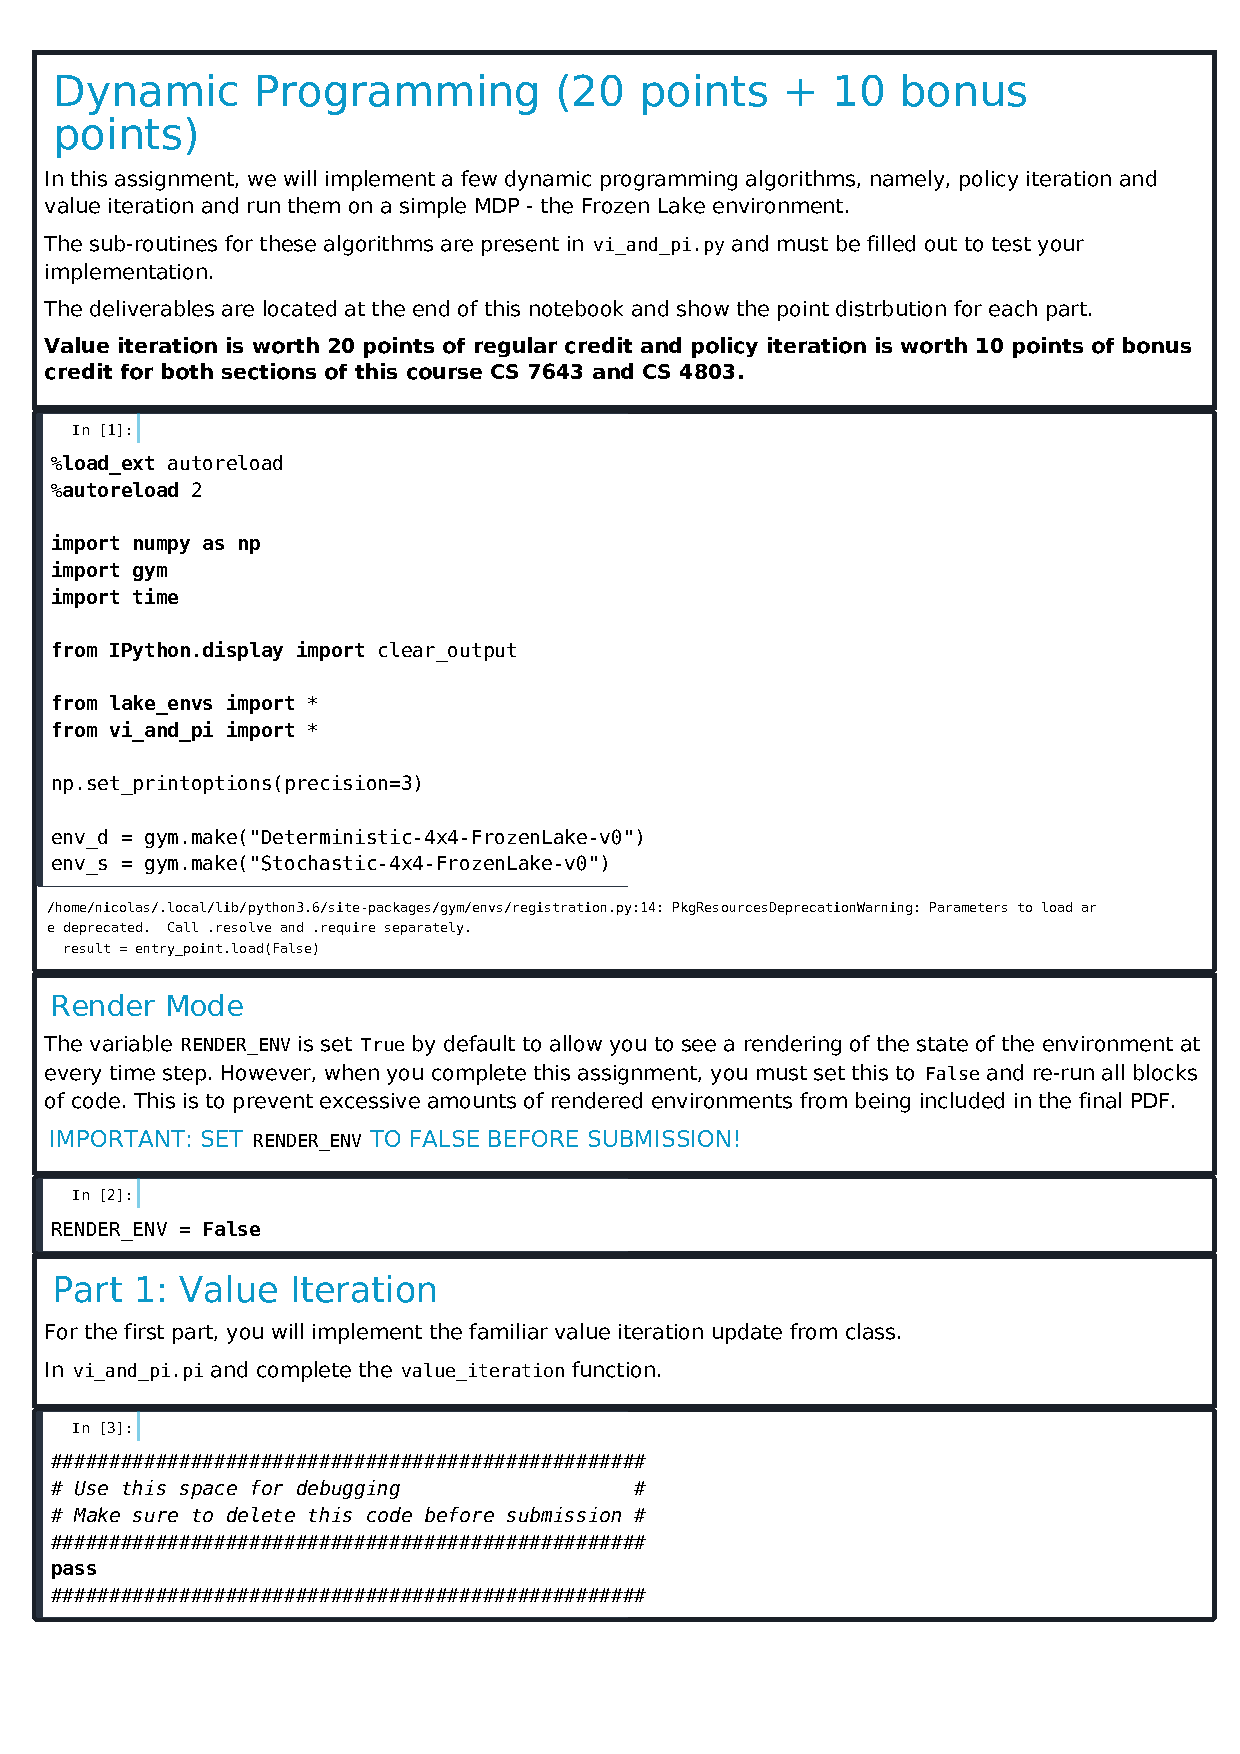
\includepdf[pages=-]{../code/dynamic_programming/dp.pdf}

    \pagebreak
    \subsection{Deep Q-Learning}
    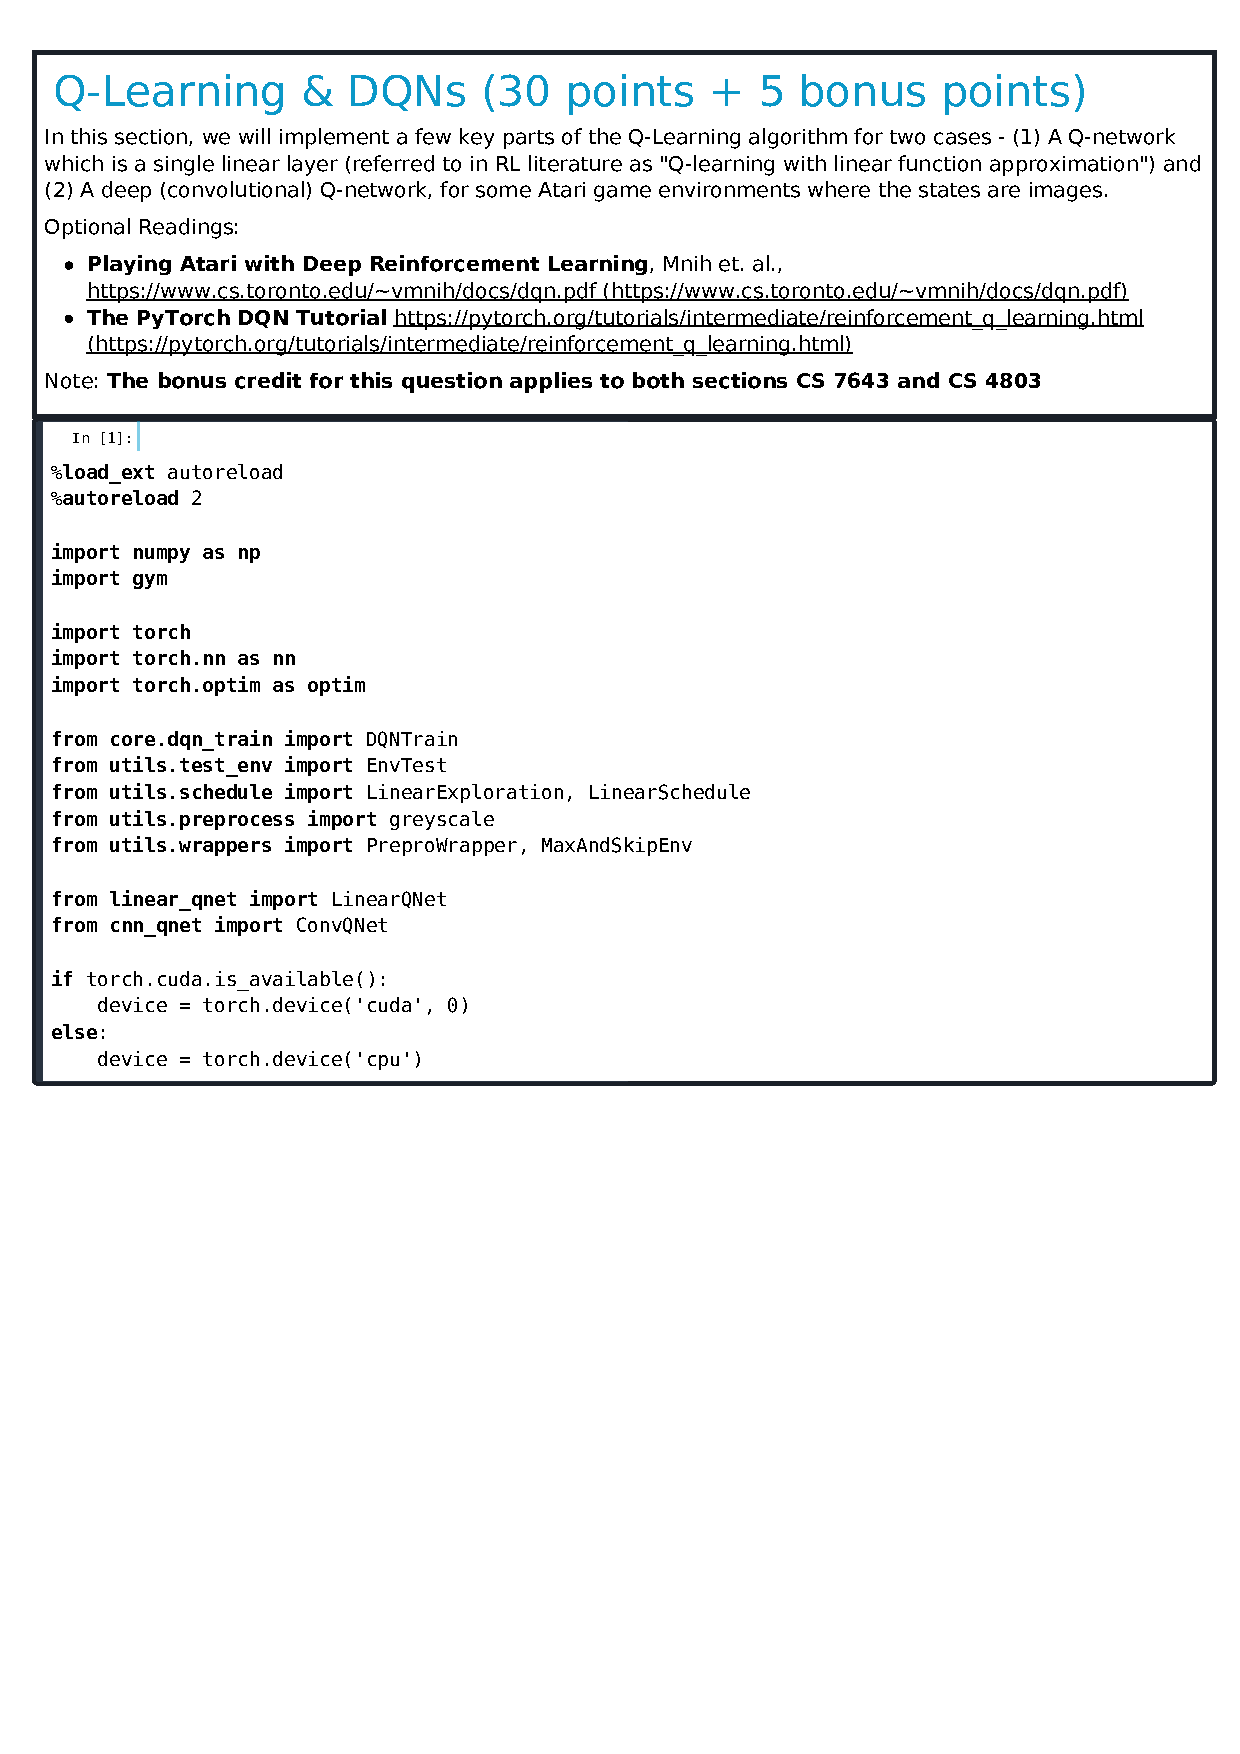
\includepdf[pages=-]{../code/q_learning/q_learning.pdf}


\end{document}
